
\documentclass{article}
\usepackage{url}
\usepackage{graphicx,subfigure}
\usepackage{xspace}

\newcommand{\ie}{{\em i.e.,}~}
\newcommand{\eg}{{\em e.g.,}~}


\title{Consumer Review Analysis with Linear Regression}

%\numberofauthors{1}
\author{Cliff Engle \and Antonio Lupher}

\begin{document}


%%%%%%%%%%%%%%%%%%%%%%%%%%%%%%%%%%%%%%%%%%%%%%%%%%%%%%%%%%%%%%%%%%%%%%%%%%%%%%%
%%%%%%%%%%%%%%%%%%%%%%%%%%%%%%%%%%%%%%%%%%%%%%%%%%%%%%%%%%%%%%%%%%%%%%%%%%%%%%%
%%%%%%%%%%%%%%%%%%%%%%%%%%%%%%%%%%%%%%%%%%%%%%%%%%%%%%%%%%%%%%%%%%%%%%%%%%%%%%%

\maketitle

\section{Introduction}
Sentiment analysis aims to classify people's sentiments towards a particular subject based on their opinions. There are a number of different classification methods that can be used to perform this analysis. In this paper, we perform sentiment analysis on a labeled dataset of Amazon product reviews using linear regression. The dataset consists of one million textual reviews, of which approximately 500,000 are unique. We perform 10-fold cross-validation of our linear regression method, and experiment with various configuration parameters to provide optimal performance.

\section{Linear Regression}
Linear regression is a method to model the relationship between an output variable, $y$, and explanatory variables, $X$. The output variable is a linear sum of the explanatory variables multiplied by their corresponding coeffecients, represented by $\beta$. In our case, $y$ represents a review's ranking from one to five, while $X$ is the bag-of-words representation of the review text. This implies that $\beta$ represents the weight of a word's correlation to a higher review. This gives us the simple regression formula: $$y=X\beta$$

In this paper, we perform ordinary least squares regression. By minimizing the sum of squared residuals, we can solve for the unkown parameter vector $\beta$ using a closed form solution. $$\beta=(X'X)^{-1}X'y$$ In order to ensure that the matrix $X'X$ is invertible, we perform ridge regression. In ridge regression, we add the identity matrix, $I$, scaled by a factor, $\lambda$, to produce the following equation. $$\beta=(X'X+\lambda I)^{-1}X'y$$ We calculate this $\beta$ for a training set of review text along with their corresponding ratings which range from 1 to 5. We then evaluate our model $\beta$ on the withheld reviews in order to perform a 10-fold cross-validation.

%%%%%%%%%%%%%%%%%%%%%%%%%%%%%%%%%%%%%%%%%%%%%%%%%%%%%%%%%%%%%%%%%%%%%%%%%%%%%%%
%%%%%%%%%%%%%%%%%%%%%%%%%%%%%%%%%%%%%%%%%%%%%%%%%%%%%%%%%%%%%%%%%%%%%%%%%%%%%%%
%%%%%%%%%%%%%%%%%%%%%%%%%%%%%%%%%%%%%%%%%%%%%%%%%%%%%%%%%%%%%%%%%%%%%%%%%%%%%%%

\section{Implementation}
All of our code was implemented in MATLAB because of its ease-of-use and optimizations on matrix multiplications. We parsed the reviews from the tokenized binary format into a bag-of-words representation stored as a sparse matrix. Matlab uses Compressed Sparse Column format, so we actually stored the matrix $X'$ because the dictionary is very sparse. We also filtered out duplicate reviews by hashing the first ten words in a review to determine distinctness. This filtered the one million reviews to 492,130.

% Talk about stemming and stop-words

The actual matrix multiplications were done using the sparse $X$ matrix along with our $y$ vector and the ridge parameter. The multiplication $X'X$ takes up too much memory if we use the entire dictionary, so we chose to limit the dictionary size. We found that a dictionary of the 10,000 most frequent words gave sufficient features while also being computable using MATLAB's built-in sparse matrix multiplications. We also tried using a dictionary of 15,000 words, but only had a marginal improvement along with much slower execution. Using our 10,000 word dictionary, we calculated the performance of our matrix multiply to be 0.123 Gflops/s by dividing the number of non-zero elements in our matrices by the time to compute the multiplication.

\section{Design Decisions}

\subsection{Tuning the Lambda parameter}
Since we used ridge regression, we had the ability to tune the $\lambda$ parameter in order to get the best performance. As shown in figure \ref{fig:lambda}, we observed an AUC improvement of about .5\% between the default value of 1 and a tuned parameter of 1500. This is a fairly major difference since the AUC is at 93\% using the default value. Additionally, we also noticed a major difference in the top words when using better $\lambda$ values. Using the default value of 1, our top words included obscure words including ``\_c'', ``\_j'', ``donovan'', and ``matlock.'' When we used the tuned $\lambda$ value of 1500, the words were much more representative, as shown in table \ref{tab:words}.

\begin{figure}[h]
	\centering
	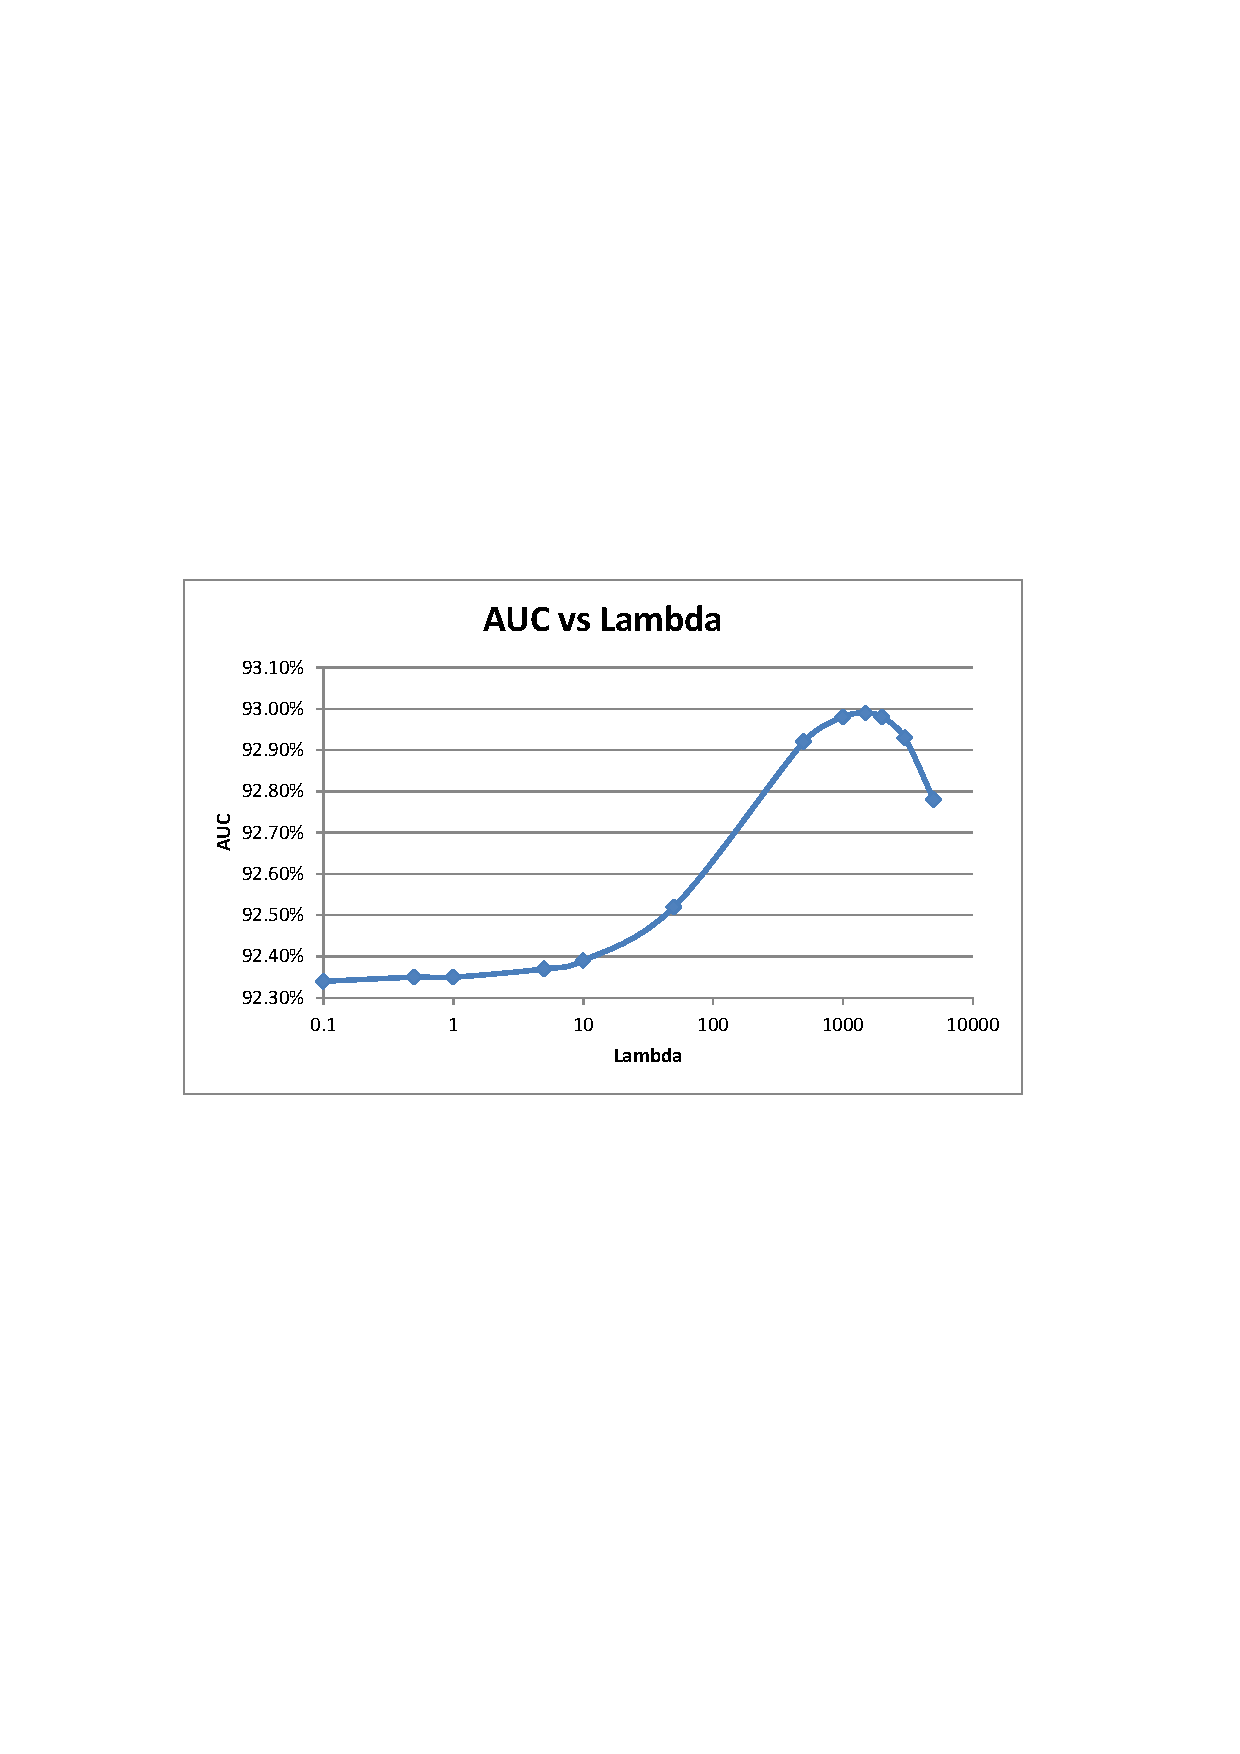
\includegraphics[width=\linewidth]{files/lambda.pdf}
	\caption{AUC based on varying lambda values for Ridge Regression. Dictionary is pruned to 15,000 words.}
	\label{fig:lambda}
\end{figure}

\subsection{Porter Stemming}
Porter Stemming is a process for removing some of the common morphological and inflexional endings from words. The ramifications of this in a classifier is that it consolidates words with similar semantics. This can often help to reduce dependencies between similar words. We ran performance tests with and without Porter Stemming. 

\subsection{Stop Words}

In order to minimize the influence of small, commonly-used words on the sentiment analysis, we tested a model that ignored a set of approximately 125 stop words. This list included words like 'the', 'and', 'a', and 'are'. However, a 10-fold cross-validation across the entire data set showed that the AUC difference between the model that omitted stop words and our base model was only 0.5\%. Likewise, the most heavily weighted terms remained almost exactly the same as for the original model.
\\\\Considering this negligible variation and the observation that no stop words appeared in our most heavily weighted positive and negative word lists, we can conclude that the effect of these common words is not substantial. This is most likely because they are for more or less evenly distributed among positive and negative reviews.


\section{Results}
The baseline results of our 10-fold cross-validation using a dictionary of 10,000 words and a $\lambda$ of 1 are an AUC of 0.9257 with a 1\% lift of 34.067. The optimal value that we achieved was using a dictionary size of 15,000 words and a $\lambda$ of 1,500, which gave us an AUC of 0.9313 and a lift of 38.27. We did not observe improvements with Porter Stemming or stop word removal, as shown in in figure \ref{fig:auc}. We also believe that a larger dictionary size offers only modest improvements, as our AUC difference between using 10,000 and 15,000 words is only .0013 when using tuned $\lambda$ parameters.

\begin{figure}[h]
	\centering
	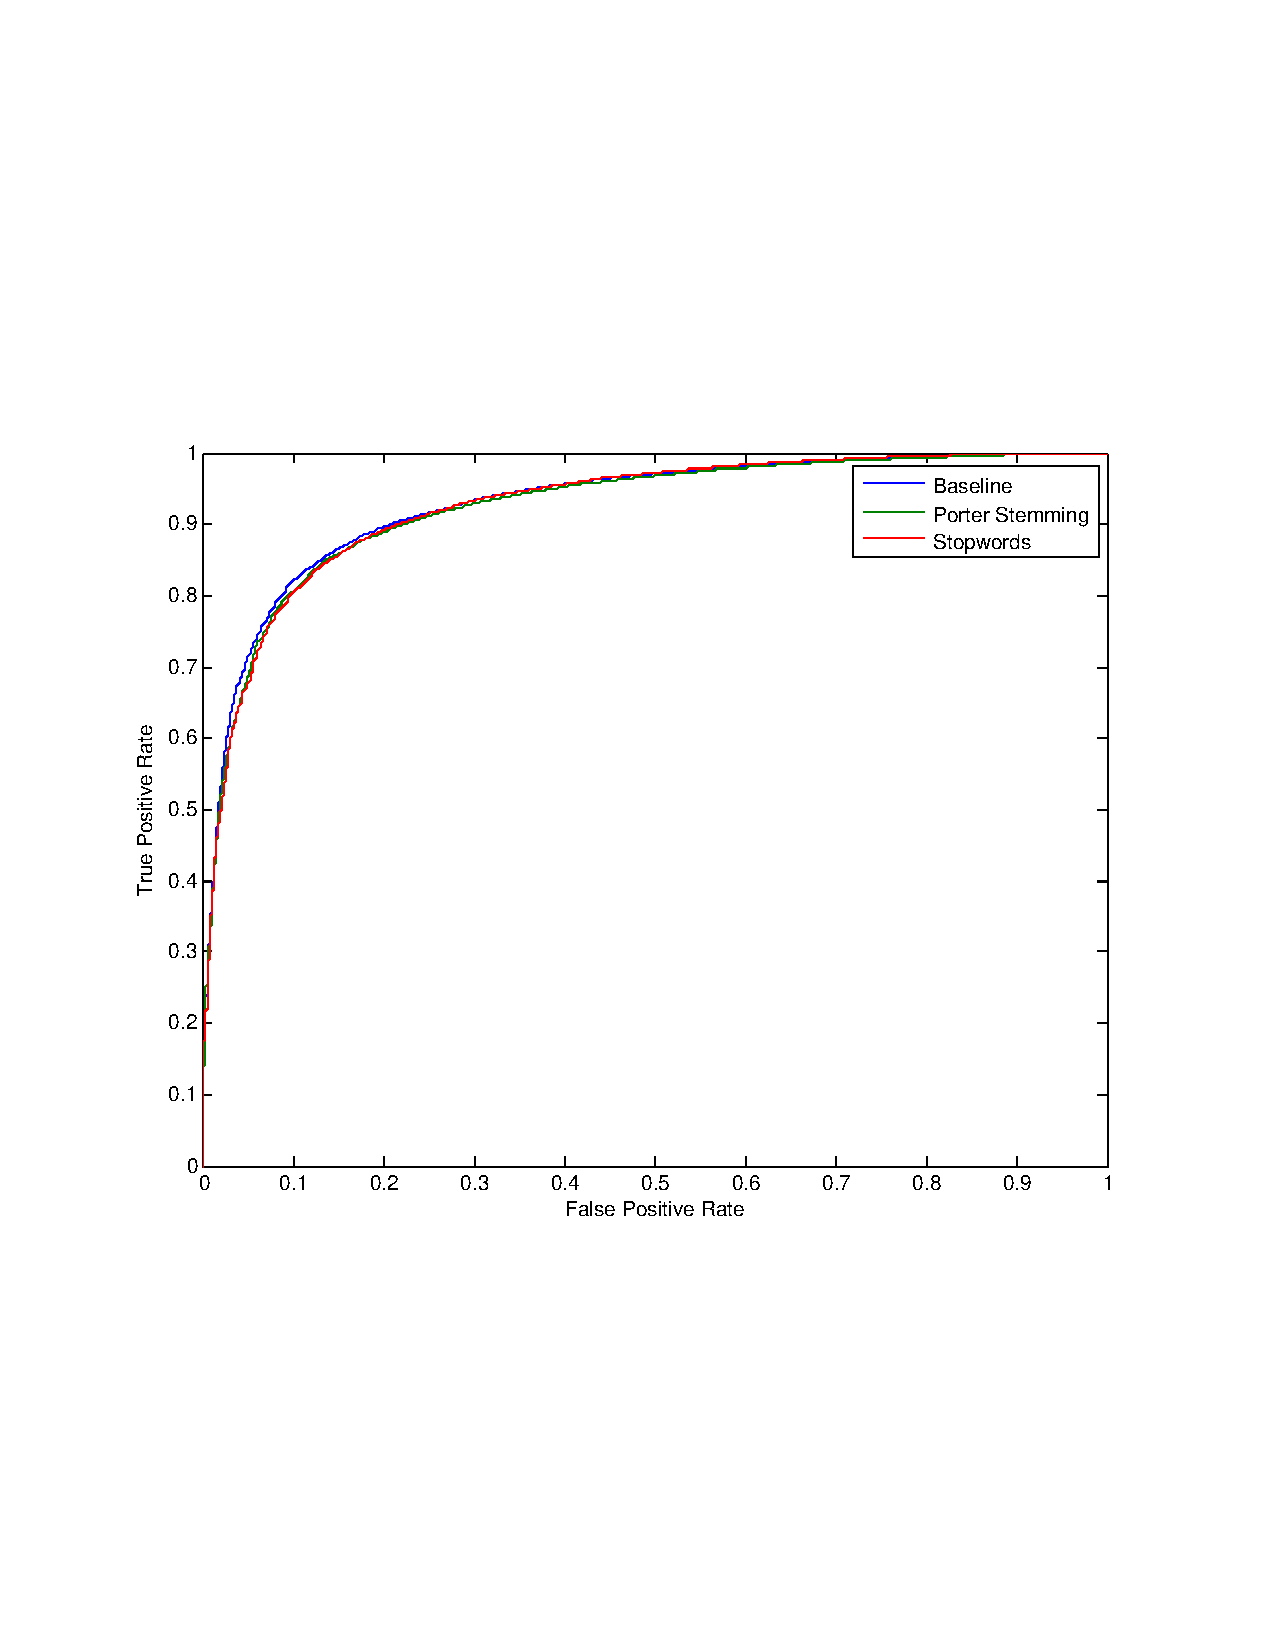
\includegraphics[width=\linewidth]{files/aucs.pdf}
	\caption{AUC for baseline, stemmed and stop word models.}
	\label{fig:auc}
\end{figure}

\section{Analysis}
\subsection{Top Words}
As mentioned above, the lambda parameter played a major role in the top words. Having a better tuned lambda gave more reasonable top words and improved performance. Looking at the words in table \ref{tab:words}, all of the top 10 positive and negative words seem quite reasonable and accurate. It is interesting to note that negative words have much stronger weights than positive words. The top negative word, ``waste'', has 3.5 times more weight than the the top positive word, ``excellent.'' This is likely due to the fact that the reviews in this dataset were heavily skewed towards being positive. The mean review rating is 4.23. 

\begin{table}[h]
    \begin{tabular}{|l|l|l|l|}
        \hline
        Top Positive Words & Weights & Top Negative Words & Weights \\ \hline
        excellent   & 0.20 & waste          & -0.71 \\ 
        awesome     & 0.18 & disappointing  & -0.57 \\ 
        invaluable  & 0.15 & poorly         & -0.56 \\ 
        highly      & 0.15 & disappointment & -0.52 \\ 
        amazing     & 0.15 & worst          & -0.47 \\ 
        outstanding & 0.15 & boring         & -0.46 \\ 
        wonderful   & 0.14 & disappointed   & -0.46 \\ 
        loved       & 0.14 & useless        & -0.42 \\ 
        pleased     & 0.14 & hoping         & -0.32 \\ 
        fantastic   & 0.14 & lacks          & -0.31 \\
        \hline
    \end{tabular}
    \caption{Top words and their weights using a lambda of 1500}
    \label{tab:words}
\end{table}


\subsection{Porter Stemming}

Adding Porter Stemming to our model did not have a significant impact on the AUC.  The 10-fold cross-validation AUC for our stemmed model was 92.5\%, which 0.5\% lower than the base line AUC. This negative impact might be due to stemming causing certain positive and negative words to be reduced to the same stem, thus lowering their influence. This lack of accuracy gain with stemming is consistent with our results in Homework 1, where stemming had a negative effect on the accuracy of our Naive Bayes sentiment classifiers.
\\\\The positive and negative stems with the most weights are slightly different and in a different order than our results above. As was expected, words with the same stem were consolidated. For example, our top negative words for the base model included 'disappointing', 'disappointment', and 'disappointed'. In the stemmed results, these separate words have been consolidated into the single stem 'disappoint', allowing new stems like 'unfortuna', 'terribl', and 'mislead' to enter the top ten negative words. Interestingly, the weight of this consolidated stem does not place it any higher than it was in the original list, presumably because the next stem, 'poor', has also gained more weight from similar consolidations.

\begin{table}
    \begin{tabular}{|l|l|l|l|}
        \hline
        Top Positive Words & Weights & Top Negative Words & Weights \\ \hline
	awesom\_book & 0.19 & wast  & -0.64 \\
	excel & 0.19 & poor & -0.57 \\
	highlif &   0.16 &  disappoint &  -0.56 \\ 
	invaluab & 0.15 & worst/best  & -0.47 \\
	amaz & 0.14 & useless/worthless & -0.41 \\ 
	superb & 0.14 & bore &  -0.30 \\
	outstand & 0.13 & sorri &  -0.27 \\
	terrifc & 0.13 & terribl & -0.27 \\
	fantasti & 0.13 & unfortuna &  -0.26 \\
	thank\_you & 0.12 & mislead &  -0.25 \\
        \hline
    \end{tabular}
    \caption{Top words with Porter Stemming and $\lambda$ = 1500}
    \label{tab:stemwords}
\end{table}

%\subsection{Dictionary Size}
%
%For the results above, we pruned the dictionary to the 15,000 most frequently-encountered words to simplify the calculations necessary to perform the regression. However, we also tested 10,000-word, 20,000-word and 25,000-word dictionaries on the dataset. For this, we used a single pair of training and validation data sets comprising 90\% and 10\% of the review corpus respectively with a random ordering of reviews. 

%\begin{table}
%    \begin{tabular}{|l|l|l|l|}
%        \hline
%        Dictionary Size & AUC \\ \hline
%        10,000   & ???  \\ 
%        15,000   & ???  \\ 
%        20,000   & ???  \\ 
%        25,000   & ???  \\ 
%        \hline
%    \end{tabular}
%    \caption{Dictionary Size vs. AUC}
%    \label{tab:dict}
%\end{table}


%%%%%%%%%%%%%%%%%%%%%%%%%%%%%%%%%%%%%%%%%%%%%%%%%%%%%%%%%%%%%%%%%%%%%%%%%%%%%%%
%%%%%%%%%%%%%%%%%%%%%%%%%%%%%%%%%%%%%%%%%%%%%%%%%%%%%%%%%%%%%%%%%%%%%%%%%%%%%%%
%%%%%%%%%%%%%%%%%%%%%%%%%%%%%%%%%%%%%%%%%%%%%%%%%%%%%%%%%%%%%%%%%%%%%%%%%%%%%%%
\section{Future Improvements}

While we were pleased that our results showed high AUC and relevant terms for the top positive and negative weights, we would expect more accurate results by incorporating bigrams as features. This would allow us to more accurately classify phrases that might have meanings substantially different from their component words. For example, 'not bad' could be correlated to positive reviews, even while 'not' and 'bad' would connote negative sentiment. Adding bigrams poses the challenge of creating a new, much larger, dictionary to keep track of the occurrence of both bigrams and unigrams.


%%%%%%%%%%%%%%%%%%%%%%%%%%%%%%%%%%%%%%%%%%%%%%%%%%%%%%%%%%%%%%%%%%%%%%%%%%%%%%%
%%%%%%%%%%%%%%%%%%%%%%%%%%%%%%%%%%%%%%%%%%%%%%%%%%%%%%%%%%%%%%%%%%%%%%%%%%%%%%%
%%%%%%%%%%%%%%%%%%%%%%%%%%%%%%%%%%%%%%%%%%%%%%%%%%%%%%%%%%%%%%%%%%%%%%%%%%%%%%%

%%%%%%%%%%%%%%%%%%%%%%%%%%%%%%%%%%%%%%%%%%%%%%%%%%%%%%%%%%%%%%%%%%%%%%%%%%%%%%%
%%%%%%%%%%%%%%%%%%%%%%%%%%%%%%%%%%%%%%%%%%%%%%%%%%%%%%%%%%%%%%%%%%%%%%%%%%%%%%%
%%%%%%%%%%%%%%%%%%%%%%%%%%%%%%%%%%%%%%%%%%%%%%%%%%%%%%%%%%%%%%%%%%%%%%%%%%%%%%%




\end{document}
